\documentclass[11pt, letterpaper, notitlepage]{article}

\usepackage{multicol}
\usepackage{fancyhdr}
\usepackage[margin=0.75in]{geometry}
\usepackage{graphicx}
\usepackage{hyperref}
\usepackage{authblk}
\usepackage{amsmath, amssymb}
\usepackage[hypcap=false]{caption}
\usepackage{float}
\graphicspath{ {./images/}}

\usepackage{biblatex}
\addbibresource{PNNL-CT.bib}

%-------------Custom Abstract Def----------------
% Modified abstract command in order to better suit the styles common in other papers in the field.
\def\abstract{\if@twocolumn
\section*{Abstract}
\else
% modified quotation macro from latex.tex
\list{}{\listparindent 1.5em \topsep 1pt \parskip 0pt \partopsep 0pt
 \itemindent\listparindent
        \setlength\rightmargin{5em}
        \setlength\leftmargin{5em}
 \parsep 0pt plus 1pt}\item[]
% end of modified quotation macro
\noindent \footnotesize{\bf Abstract.}
 \ignorespaces %  -SLK-00Mar12> 
\fi}
\def\endabstract{\if@twocolumn\else\endlist\fi\bigskip\smallskip}

%-------------Title Details----------------------
\title{%
  Quantitative Analysis for Computed Tomography\\
  \large \vspace{1em}\textbf{Stage 2 Progress Report}
}

%\author[1]{Thomas Pasfield}

\author{Yianni Parachos}
\author{Thomas Pasfield}
\author{Kian Greene}
\author{Dylan Pereira}
\author{Ryan Reynolds}
\author{Jacob Koscinski}

\affil{Embry-Riddle Aeronautical University, Daytona Beach, FL.}

% Industry Partners (: Finally fixed the footnote!)
\affil{\small Industry Representatives: Aaron Luttman\footnote{Pacific Northwest National Laboratory Richland, WA.}\;, Margaret Lund$^*$}

%-------------Header/Footer Modification---------
\pagestyle{fancy}
\fancyhead{}
\fancyhead[L]{Quantitative Analysis for CT}
\fancyhead[R]{\thepage}
\fancyfoot{}
\setlength{\headheight}{13.59999pt}
\addtolength{\topmargin}{-1.59999pt}


\newenvironment{Figure}
  {\par\medskip\noindent\minipage{\linewidth}}
  {\endminipage\par\medskip}

\begin{document}
\maketitle

%\begin{abstract}
%\end{abstract}

\begin{multicols}{2}
\section{Background}
  \subsection{Industrial Partner}
    The Pacific Northwest National Laboratory (PNNL) is a U.S. Department of Energy research lab that specializes in nuclear and material science. They have been located in Richland, WA, since the lab's inception in 1965. Over the decades, they have diversified from nuclear weapons research to medicine, biology, environmental science, and more.\cite{noauthor_national_nodate} To improve material analysis methods and support the proliferation of additive manufacturing in the precision industry, the lab wishes to implement Computed Tomography (CT).

  \subsection{What is Computed Tomography?}
    Computed Tomography is a method of 3D analysis of internal and external structures using X-ray images. It consists of imaging X-ray transmission through an object at various angles. 3D data is represented as "voxels," which are the 3D analogs of pixels. The voxel format of the data is generated from the transmission images via the Radon transform.

    CT scanning is most common in medical imaging and widely used in industrial applications. It can analyze assemblies, single objects, and internal structures. The state-of-the-art is working towards precise object dimensioning and internal defect detection.

\section{Scope of the Problem}
%This project requires our talents to enhance the processing and visualizing of CT data, which presents many of the challenges we would be facing while attempting to accomplish the company's task given to us. The first task that helped us move forward with the project was visualizing the TIFF file data type; doing so would help accomplish our main objective. 

% The main objective is to generate 2D and 3D images, needing a lot of programming and mathematics expertise in the team the project seeks. With the images, it moves to the printing phase as we go steeper. Having the results from the CT scan, we need to differentiate between the three materials, giving us the data for it.This task would require most of our time and precision to generate data results from CT scans. It won't be an easy task for us to accomplish this promptly. Still, thankfully, with our industrial partner and many talented students, we anticipate that we will be able to accomplish the project task, which will fulfill the objective of implementing CT in their laboratory. 
% Draft By Dylan L Pereira
% Needs completion
% Mention image dimensions/quantity

CT as a technology has found wide application in the biomedical sector and growing application in the industrial sector. Our work will specifically pertain to the industrial sector. It will explicitly focus on developing and implementing methods specific to the analysis of additive-manufactured components. 

In this application, our goals include object dimensioning, defect detection/dimensioning, layer cohesion, infill structure analysis, and material identification/segmentation. This work is intended to explore the state-of-the-art and bring various approaches together cohesively. The work may aid in standardizing and certifying CT as a trusted tool in precision manufacturing.

\section{Data Visualization}
% Some images that could go here will be cited and placed in the Appendix, as they are unsuitable for the 2-column format. 
One of the first issues we encountered with data visualization was the data type used within the TIFF files. Though TIFF has supported 32-bit floating point values for at least 22 years, most photo viewers do not support this precision. To aid in our work, reduce strain on code, and generally make the data more intuitive, we have normalized the image data to an 8-bit unsigned integer depth. The difference between the value spread of the raw and normalized data is shown in Figure \ref{fig:comphist}.

\begin{Figure}
    \centering
    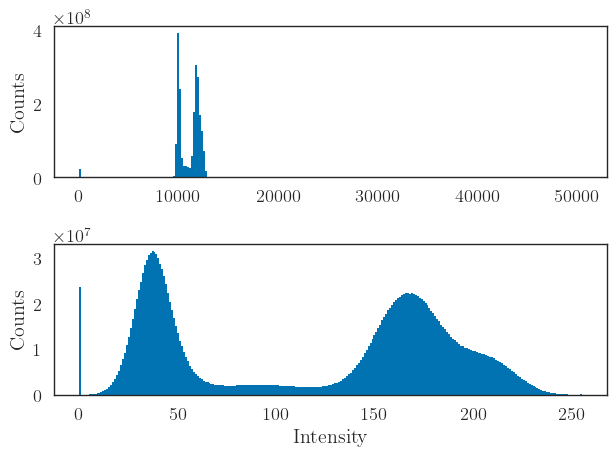
\includegraphics[width=3in]{images/hist-compare.png}
    \captionof{figure}{\emph{A comparison of the voxel intensity distributions of the raw and the normalized data.}}
    \label{fig:comphist}
\end{Figure}


Even at full precision, MATLAB\cite{inc_matlab_2022} is a fast, though not exceptionally reliable, tool for data visualization. Setting up and installing the proper toolkit to use the \verb|VolumeViewer| function is easy. This viewer allows for easy point cloud visualization and easy modification of the thresholds, transparency, and other parameters that are useful for visual analysis. A screenshot of the 3D window of \verb|VolumeViewer| is seen in Figure \ref{fig:mat3d}.

\begin{Figure}
  \centering
  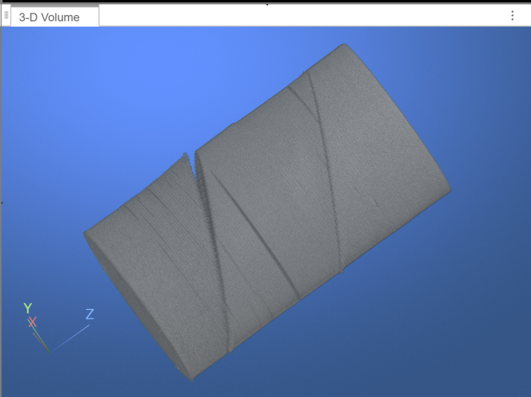
\includegraphics[width=3in]{images/MATLAB_VV_2D.png}
  \captionof{figure}{\emph{Early visualization of the voxel image using MATLAB's Volume Viewer that comes with Mathworks' Image Processing Toolbox.}}
  \label{fig:mat3d}
\end{Figure}

% RegularImageJ
In addition, the image analysis application ImageJ was used to visually inspect the data while still in its 2-D form.  By loading all of the images into the ImageJ interface as an "image stack", it was possible to visualize the internal structure of the entire 3-D object by quickly cycling through the 2-D slices. Doing this grants us a number of advantages regarding analysis of the object, as well as the 3-D printing process.  By cycling through the slices in the stack, we could, in a sense, "scan" up and down through the object, revealing each layer of 3-D printed material. The following figure shows one of the many 2-D slices that we were able to visualize through ImageJ:
% Temporarily removing ImageJ image since Ryan is much better at using it than I am. I'll leave ImageJ's inclusion to him.
\begin{Figure}
  \centering
  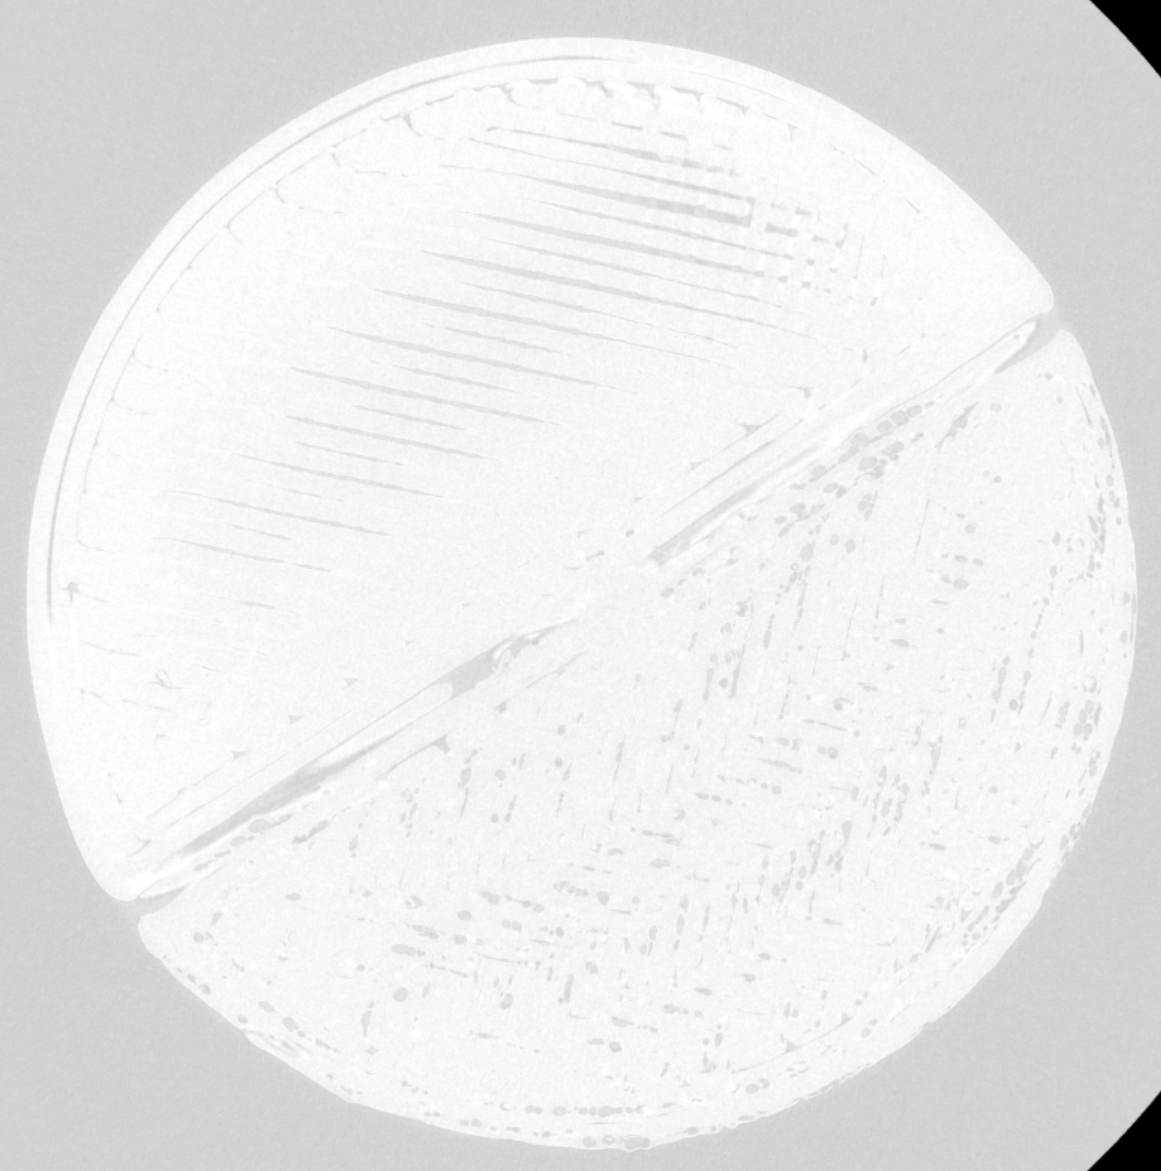
\includegraphics[width=3in]{images/CTscan.png}
  \captionof{figure}{\emph{A 2-D slice of the object visualized using ImageJ, which features a portion in which two materials meet.  Note the visibility of the two materials, and how the 3-D printing quality differs for each.}}
  \label{fig:imj2d}
\end{Figure}

As shown in the figure, the 2-D visualization of the slices allowed us to see how the 3-D printing process deposits the different layers for each material as well as the internal quality and integrity of each 3-D printed material in its respective section of the object. In this specific image, it is clear that the material in the top half of the slice is more yielding to the 3-D printing process than the material used for the bottom half.

% AstroImageJ
AstroImageJ was also considered due to its different visualization features aside from ImageJ. In particular, we used the interactive 3D surface plots to map the relative intensity of the X-rays through the different materials, which also helped visualize the separation gap between them. In particular, the example slice shown in Figure \ref{fig:aij3dline} and \ref{fig:aij3disoline} the polylactic acid and polycarbonate sections of the object, which composed the top section and the middle section, respectively.

% NOTE: Determine what slice number was used for this AstroImageJ example (for clarity)

\begin{Figure}
  \centering
  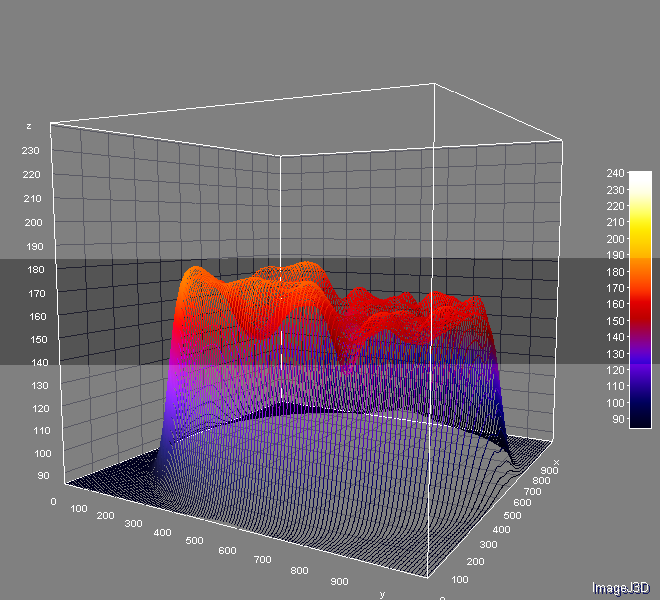
\includegraphics[width=3in]{images/Norm_Slice_Line_Plot_Angled.png}
  \captionof{figure}{\emph{Angled view of an example AstroImageJ slice with normalized intensities given by the color map on the right side of the image. Here, there is a significant valley in the middle of the plot that corresponds to the gap between different materials.}}
  \label{fig:aij3dline}
\end{Figure}

\begin{Figure}
  \centering
  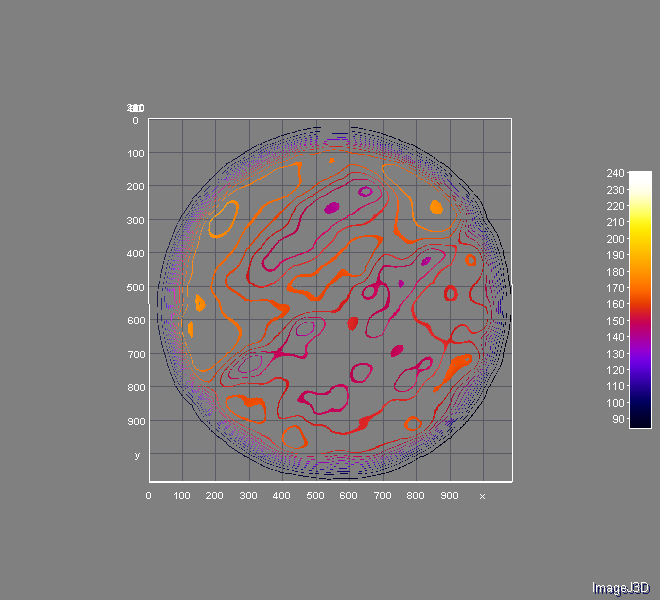
\includegraphics[width=3in]{images/Norm_Slice_Isoline_Plot_Top-Down.png}
  \captionof{figure}{\emph{Top-down view of the same AstroImageJ slice as Figure \ref{fig:aij3dline} with normalized intensities given by the color map on the right side of the image. Here, the isoline viewer was used to account for the top-down view of the slice.}}
  \label{fig:aij3disoline}
\end{Figure}

%% PYTHON DATA VIS, TJ covering initial methods, 2D, and ITK. Yianni, please add your grid image here, along with any relevant info. 
Python proved to be a much higher-performing and more reliable solution for visualization. The \verb|matplotlib|\cite{hunter_matplotlib_2007} library provided extensive options and customization for data visualization in 1D and 2D. This works regardless of the precision format, which makes it incredibly useful. The code was easy to use, reasonably efficient, and very modular. Figure \ref{fig:comphist} utilized this library for its generation.

Additionally, Python has an extensive wrapper for Insight Toolkit (ITK)\cite{mccormick_itk_2014}. ITK is a scientific image-processing library with extensive support and features related to our work. Within it exists a module called \verb|itkwidgets|, which adds interactive 3D visualization support. This was quite useful for the initial viewing of the data and evaluation of the normalization and down-sampling techniques. A screenshot of this visualization and its interface is in the Appendix in Figure \ref{fig:itk}.

\section{Initial Strategy}
% Yianni
Initially, the object will be analyzed slice by slice. By analyzing a single slice, an algorithmic process can be developed to analyze relevant features of the object. Relevant features include: voxel intensity, distance between the infill layers via voxels, and deformation and separation of each material. 

By viewing a histogram of the intensity of pixels through each image, the bounds of what are considered "air" and "object" can be clearly defined. Because each of the materials hold a different intensity, the bounds of each object's "brightness" can be documented. This can be used to differentiate objects algorithmically, even when multiple materials are present within an image. 

After analysis of the images directly, the images will be segmented so that they are binarized. This allows us to distinctly separate 'air' and 'object' within each image to measure infill separation and material deformation. To perform this effectively, this must be done on images with individual materials and then applied to images with multiple included materials. 

\section{Metrology Methods}
Our early dimensioning approaches are fueled almost purely by intuition rather than current literature. We are working on getting an intuitive grasp of the problem among our members. Once achieved, we will broaden our work towards directly implementing and applying existing methods. That being said, we believe that our preliminary results have some merit.

\subsection{Approach \#1}
Thomas' initial approach builds from his previous experience with OpenCV\cite{opencv_library}. The approach is split into two processes, the first determining the height and the second determining the diameter. This order was selected to improve the diameter step since the upper and lower boundaries have diameter measurements that are significant outliers.

The height detection method consists of processing line-outs of each column along the z-axis. These line-outs plot the intensity relative to the object's depth, where the bounds are quite clear visually. This opens two approaches, both unfortunately susceptible to variability and noise. In one approach, the upper and lower bounds can be determined by iterating from each respective edge of the image until the intensity passes a set threshold. This can define an edge. The results of this method can be seen in Figure \ref{fig:height}.

\begin{Figure}
  \centering
  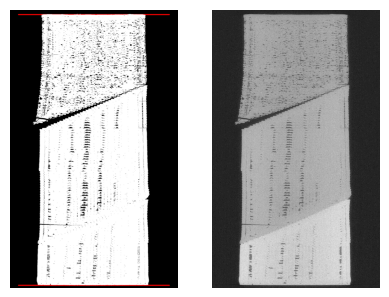
\includegraphics[width=3in]{images/height-fit.png}
  \captionof{figure}{\emph{Example slice and overlay after the height approximation method is performed. The upper and lower bounds are determined separately, approaching the object from their own edges.}}
  \label{fig:height}
\end{Figure}

The other height analysis method follows a similar approach but uses the 1st-order derivative of the line-out. The same iteration process is used, but the threshold is set to find a significant enough change. No real difference in output was found between these methods. Faster performance is achieved without performing the discrete derivative.

After the height detection method is performed across all line-outs, the data has some distinct outliers from regions of the image where the object is not present. These outliers are removed from the data by determining the standard deviation and the distance of each value from the median. The final height determination is the mean of the trimmed dataset.

The diameter detection is where it gets a little more convoluted. A Canny edge detection is performed on each slice to generate a binary mask of edge locations. An additional mask is generated using OpenCV, tracing a circle with the center coordinates and the radius as input parameters. These two masks are compared using a logical `and' operation, and the sum is returned as part of a cost function. This cost function is provided, along with guess inputs, into the \verb|scipy.optimize.fmin()| method to quickly determine the best-fit circle.

The radii determined by this method are then gathered, and outliers are removed (this time with the help of knowing the height). Doubling these values gives an estimate of the diameter. It is important to note that this output diameter only can be an even integer (in voxels). It can only increment by $\pm 40.8764 \mu$m in metric. This is a significant downside to this method. This method is demonstrated in Figure \ref{fig:circlefit}.

\begin{Figure}
  \centering
  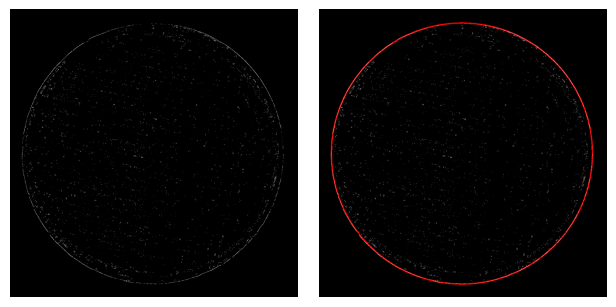
\includegraphics[width=3in]{images/circle-fit.png}
  \captionof{figure}{\emph{The edge-detected slice and the circle overlay shown side-by-side. The circle was fit to the edges using a custom cost function.}}
  \label{fig:circlefit}
\end{Figure}

Possible improvements to this method may be found through a graphics library that supports sub-pixel center locations, floating point radii, and anti-aliased outlines. Employing a new edge detection method, such as Sobel, may also improve results if these changes are made, as they might have more gradient data that preserves information.

\section{Next Steps}
% Anyone can help with this section. 
Upcoming progress for our work is currently focusing on the understanding of segmentation. Figure \ref{fig:comphist} shows that the intensity distribution resembles a Gaussian mixture distribution. There is a clear gap between the background and presumed object material intensities, though there is an unusual plateau between them. Perhaps some combination of voxel location and the intensity's relation to the Gaussian may aid in the material determination. 

The Gaussian mixture can have its components fit using \verb|scikit-learn|'s statistics tools. Precisely, the \verb|GaussianMixture| method. This tool allows for the division of the distribution into its principal components. The number of components can be specified based on intuition or determined quantitatively. Intensity values can be input once the model is created with those components. The model will then return confidence values for each of the curves.

Further development and refinement of dimensioning methods are expected in the coming weeks as well, especially as the knowledge base of members grows. Work may be split based on interest, such as delegating work on defect detection to specific members. Preliminary work on defect, separation, and infill analysis is necessary and should start within the next two weeks.

\printbibliography

\end{multicols}

\section{Appendix}
\begin{Figure}
  \centering
  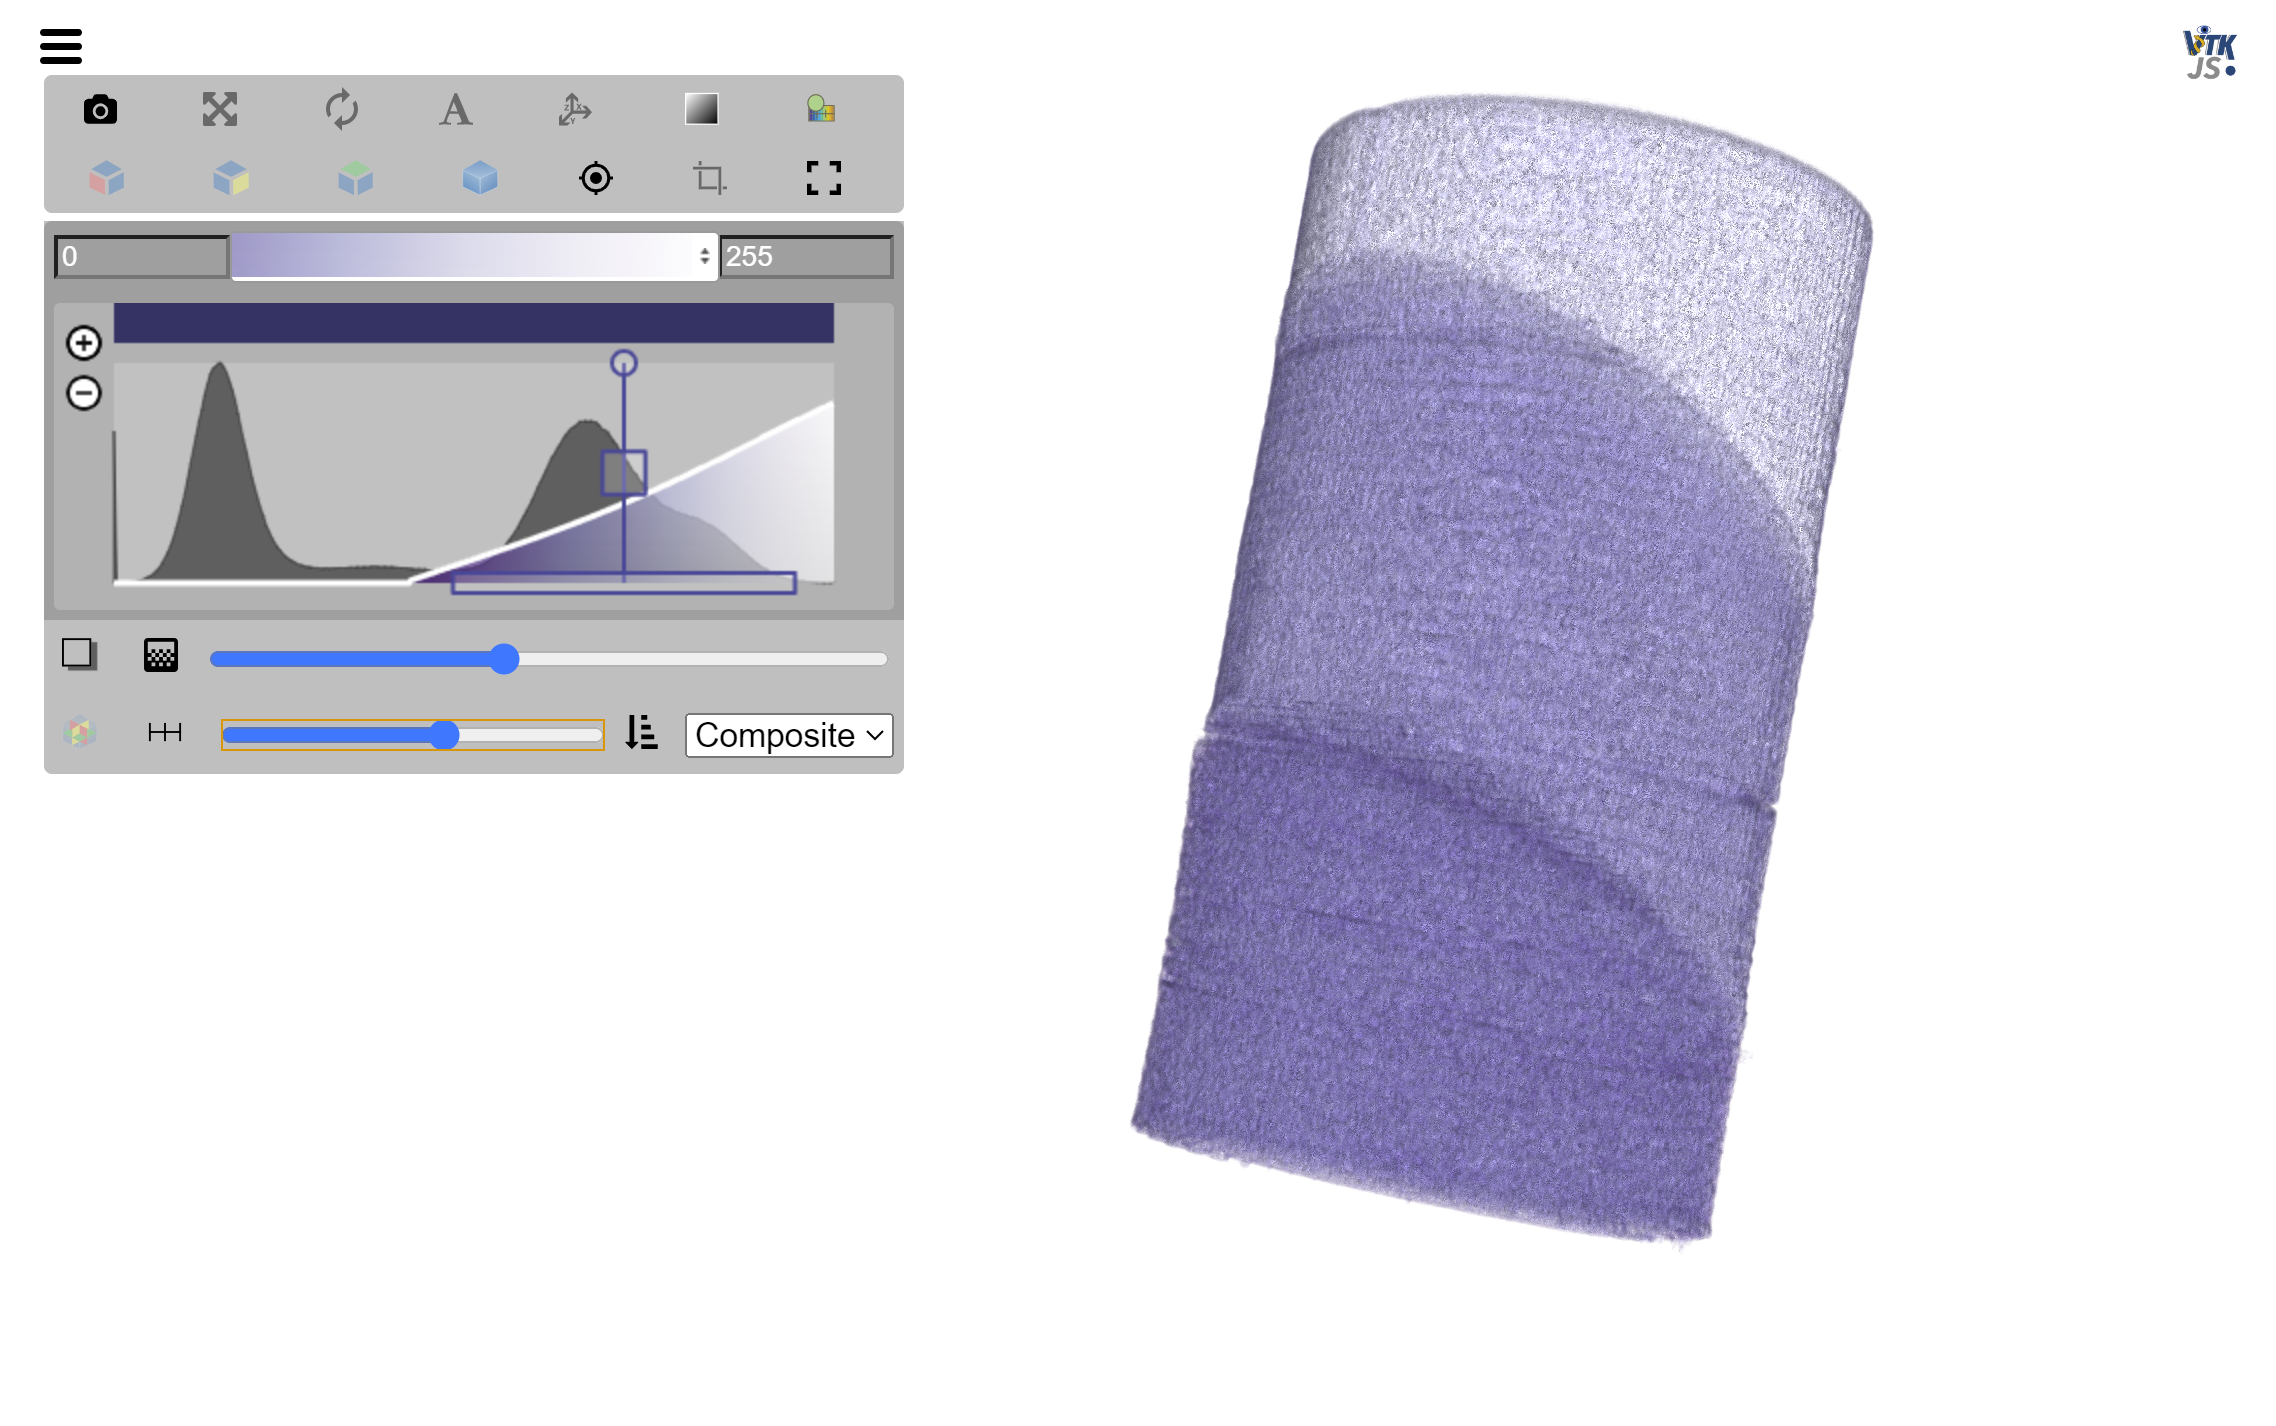
\includegraphics[width=6in]{images/itk.png}
  \captionof{figure}{\emph{The normalized dataset loaded into ITK's itkwidgets viewer tool.}}
  \label{fig:itk}
\end{Figure}
\end{document}

% PLACEHOLDERS FOR FUTURE FIGURES
%\begin{Figure}
%  \centering
%  \includegraphics[width=3in]{esf}
%  \captionof{figure}{A demonstration of the process of determining an ESF from an image. Notice the width of the blur in the image and how it relates to the edge spread shown in the ESF plot. Note that these are optimal examples without any noise present.}
%  \label{fig:ESF}
%\end{Figure}


%\vspace{1em}
%\begin{Figure}
%  \centering
%  \begin{tabular}{r|r|r|r|r|r|r}
%         & 128$^2$ & 256$^2$ & 512$^2$ & 1024$^2$ & 2048$^2$ & 4000$^2$ \\ \hline \hline
%      Half & 0.5 GB & 8.6 GB & 137.4 GB & 2199.0 GB & 35184.4 GB & 512000.0 GB \\
%      Single & 1.1 GB & 17.2 GB & 274.9 GB & 4398.0 GB & 70368.7 GB & 1024000.0 GB \\
%      Double & 2.1 GB & 34.4 GB & 549.8 GB & 8796.1 GB & 140737.5 GB & 2048000.0 GB
%  \end{tabular}
%  \captionof{table}{A table showing the size requirements for storing matrices of various sizes and precision in memory. Its exponential growth presents a significant problem for execution. The final column represents the size of image that the Cygnus x-ray machine takes. The memory capacity needed to utilize the linear model on the full data greatly exceeds any machines that we have access to, and even that of many of the world's supercomputers.}
%  \label{tab:size}
%\end{Figure}